\chapter{Analyse et spécification des besoins}

\section{Présentation du système}

Le système à développer, intitulé \textbf{Gestion des Consultations Médicales}, est une application web destinée à un cabinet médical. Il centralise l'ensemble des données relatives aux patients, aux médecins et aux consultations, et remplace la gestion manuelle par un outil unique, structuré et sécurisé.

L'application s'articule autour de deux espaces de travail distincts :

\begin{itemize}
    \item un \textbf{espace administrateur}, qui gère le référentiel complet : les patients, les médecins, les consultations ainsi que le tableau de bord ;
    \item un \textbf{espace médecin}, qui donne à chaque praticien accès à son propre planning, à son historique de consultations et à la saisie du diagnostic et de la prescription.
\end{itemize}

L'accès à l'application est conditionné par une authentification (email et mot de passe) et par le rôle de l'utilisateur.

\section{Identification des acteurs}

Un acteur représente un rôle joué par une entité (personne ou système) qui interagit avec le système. Trois acteurs principaux ont été identifiés, auxquels s'ajoute l'utilisateur non authentifié qui ne peut accéder qu'à la page de connexion.

\begin{table}[H]
\centering
\begin{tabularx}{\textwidth}{l X}
\toprule
\textbf{Acteur} & \textbf{Description et fonctionnalités principales} \\
\midrule
Administrateur &
Gère les patients (ajout, modification, suppression, recherche) ; gère les médecins (ajout, modification, suppression, filtrage par spécialité) ; planifie, modifie et annule les consultations ; consulte le tableau de bord ; accède à l'ensemble des modules après authentification. \\
\addlinespace
Médecin &
Se connecte à l'application ; consulte son planning (ses propres consultations) et son historique ; établit le diagnostic et la prescription d'une consultation ; modifie le statut d'une consultation. \\
\addlinespace
Utilisateur non authentifié &
Accède uniquement à la page de connexion ; ne peut utiliser aucune fonctionnalité métier tant qu'il ne s'est pas identifié. \\
\bottomrule
\end{tabularx}
\caption{Identification des acteurs du système}
\label{tab:acteurs}
\end{table}

Il convient de noter que le \textbf{patient} est une entité métier du système (il possède un dossier médical) mais n'est pas, dans cette version de l'application, un acteur disposant d'un espace de connexion propre.

\section{Besoins fonctionnels}

Les besoins fonctionnels décrivent ce que le système doit permettre de faire. Ils sont regroupés par module.

\subsection{Gestion des patients}

\begin{itemize}
    \item Ajouter un patient (nom, prénom, date de naissance, sexe, CIN, téléphone, email, adresse) ;
    \item afficher la liste paginée des patients ;
    \item modifier les informations d'un patient ;
    \item supprimer un patient avec confirmation ;
    \item rechercher un patient par nom, prénom ou CIN ;
    \item consulter la fiche d'un patient avec l'historique de ses consultations ;
    \item alerter l'administrateur si le CIN saisi existe déjà, afin d'éviter les doublons.
\end{itemize}

\subsection{Gestion des médecins}

\begin{itemize}
    \item Ajouter un médecin (nom, prénom, spécialité, numéro d'ordre, téléphone, email) ;
    \item afficher la liste des médecins ;
    \item modifier les informations d'un médecin ;
    \item supprimer un médecin avec confirmation ;
    \item filtrer les médecins par spécialité ;
    \item rechercher un médecin par nom ;
    \item consulter la fiche d'un médecin avec la liste de ses consultations.
\end{itemize}

\subsection{Gestion des consultations}

\begin{itemize}
    \item Planifier une consultation en choisissant un patient, un médecin, une date, une heure et un motif ;
    \item afficher la liste des consultations triée par date ;
    \item modifier ou reprogrammer une consultation ;
    \item annuler ou supprimer une consultation ;
    \item empêcher la planification de deux consultations au même créneau pour un même médecin ;
    \item empêcher la planification d'une consultation à une date passée ;
    \item permettre au médecin d'établir le diagnostic et la prescription d'une consultation ;
    \item changer le statut d'une consultation (planifiée, terminée, annulée) ;
    \item filtrer les consultations par date, médecin, patient ou statut ;
    \item prévenir l'administrateur lors de la suppression d'un patient ou d'un médecin ayant des consultations.
\end{itemize}

\subsection{Tableau de bord et ergonomie}

\begin{itemize}
    \item Proposer un menu de navigation clair ;
    \item afficher des messages de succès et d'erreur pour informer l'utilisateur du résultat de ses actions ;
    \item valider les formulaires (champs obligatoires, formats de l'email et du téléphone) ;
    \item fournir un tableau de bord (nombre de patients, de médecins, consultations du jour) ;
    \item offrir une interface responsive.
\end{itemize}

\subsection{Authentification et espace médecin}

\begin{itemize}
    \item Permettre à l'administrateur et au médecin de se connecter avec un identifiant et un mot de passe ;
    \item restreindre les fonctionnalités selon le rôle (administrateur ou médecin) ;
    \item permettre au médecin de consulter uniquement ses propres consultations.
\end{itemize}

\section{Besoins non fonctionnels}

Les besoins non fonctionnels précisent les qualités attendues du système, indépendamment des fonctionnalités.

\begin{itemize}
    \item \textbf{Sécurité} : authentification obligatoire, mots de passe, contrôle des accès selon le rôle ;
    \item \textbf{Intégrité des données} : contraintes d'unicité (CIN, email, numéro d'ordre), clés étrangères et champs obligatoires garantis au niveau de la base de données ;
    \item \textbf{Performance} : affichage paginé des listes et requêtes ciblées afin de maintenir des temps de réponse corrects ;
    \item \textbf{Ergonomie} : navigation intuitive, messages de retour, validation des saisies et interface responsive ;
    \item \textbf{Maintenabilité} : architecture en couches et séparation des responsabilités (DAO, service, contrôleur, présentation) ;
    \item \textbf{Portabilité} : utilisation de technologies JEE standard, déployables sur un serveur d'applications Tomcat.
\end{itemize}

\section{Règles de gestion}

Les règles de gestion traduisent les contraintes métier que le système doit faire respecter.

\begin{itemize}
    \item \textbf{RG1} : le CIN d'un patient et l'email d'une personne doivent être uniques ;
    \item \textbf{RG2} : les champs nom, prénom, date de naissance, sexe, CIN et téléphone d'un patient sont obligatoires ;
    \item \textbf{RG3} : la date de naissance doit être antérieure à la date du jour ;
    \item \textbf{RG4} : une consultation ne peut pas être planifiée dans le passé ;
    \item \textbf{RG5} : un médecin ne peut pas avoir deux consultations au même créneau ;
    \item \textbf{RG6} : le statut initial d'une consultation est « Planifiée », les autres statuts possibles étant « Terminée » et « Annulée » ;
    \item \textbf{RG7} : la suppression d'un patient ou d'un médecin possédant des consultations doit être précédée d'une confirmation, afin d'éviter toute perte de données ;
    \item \textbf{RG8} : l'accès aux fonctionnalités est conditionné par le rôle de l'utilisateur connecté.
\end{itemize}

\section{Diagramme de cas d'utilisation}

Le diagramme de cas d'utilisation (figure~\ref{fig:use-case}) représente les interactions entre les acteurs et les principales fonctionnalités du système. Il met en évidence la répartition des cas d'utilisation entre l'administrateur et le médecin.

\begin{figure}[H]
\centering
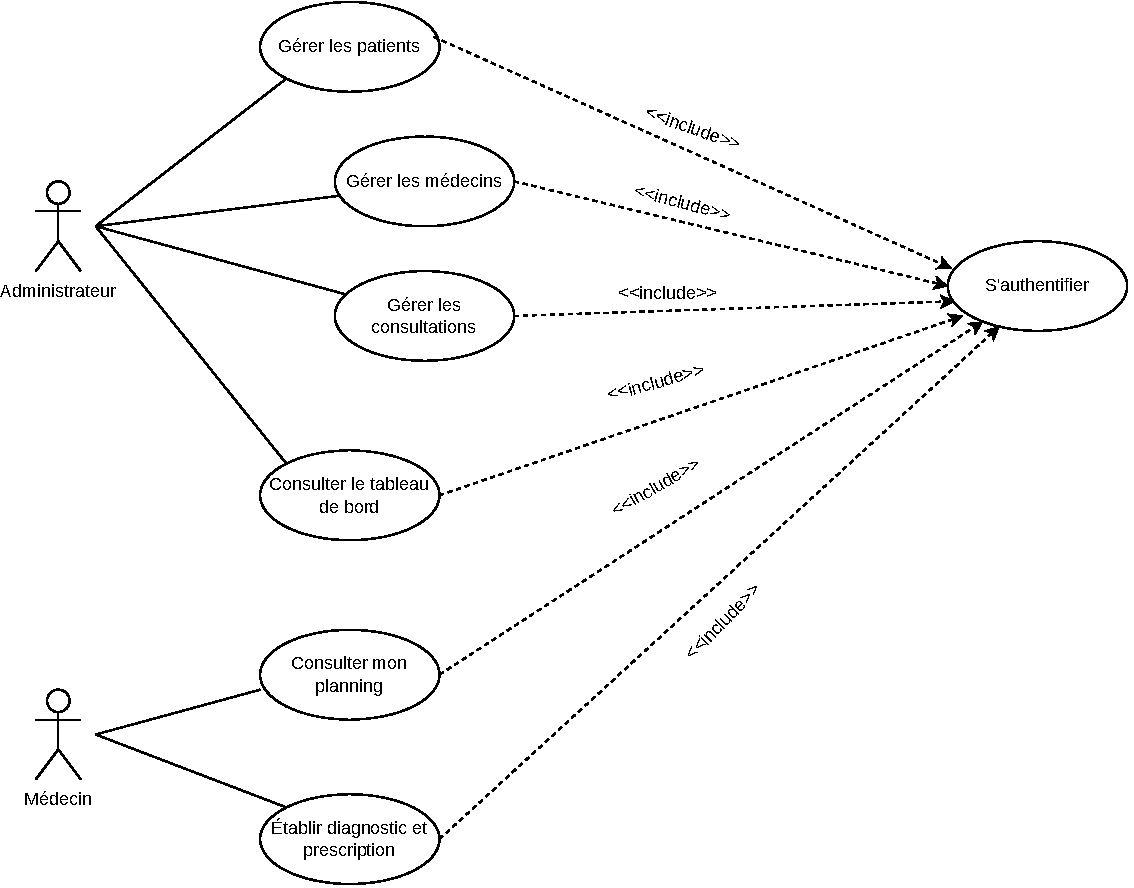
\includegraphics[width=\textwidth]{images/diagramme-cas-utilisation}
\caption{Diagramme de cas d'utilisation du système}
\label{fig:use-case}
\end{figure}

Le diagramme répartit les cas d'utilisation entre les deux acteurs. L'administrateur dispose des cas « Gérer les patients », « Gérer les médecins », « Gérer les consultations » et « Consulter le tableau de bord ». Le médecin, quant à lui, dispose des cas « Consulter mon planning » et « Établir diagnostic et prescription ».

Le cas « S'authentifier » constitue le point d'entrée obligatoire de l'application : il est inclus (relation \texttt{<<include>>}) par chacun des cas d'utilisation métier, car toute action suppose que l'utilisateur soit préalablement authentifié.
